\chapter{Particle Flow Reconstruction}

One of the goals of this thesis was to check the results of Particle Flow in Run 2 data. Therefore this chapter will give an overview of the results that the new algorithm has brought for Run 1 in data MC comparison. Before showing the results this chapter gives a description of the algorithm based on the Particle Flow Paper \cite{pflow16}. Then an update on how the algorithm has evolved is given before finally a bief overview of the results is presented.

\section{The Particle Flow Algorithm}

Recently only either the Calorimeter or the tracker information was used to reconstruct Jets in ATLAS events. The Particle Flow algorithm now combines tracker and calorimeter information to achieve better resolution especially at lower energies. The main advantages of including the tracker information into reconstruction are as follows:


\begin{itemize}
\item For low energy charged particles the momentum resolution of the tracking detector is superior to the calorimeter.
\item The tracking detector is able to reconstruct soft particles, which would not pass the noise threshold of the calorimeter.
\item The ATLAS tracking detector has a superior angular resolution for single charged particles.
\item Low $p_T$ charged particles may be swept out of the cone before reaching the calorimeter by the magnetic field. The tracker information allows to cluster these particles into the jet.
\item a better vertex determination could lower the pileup-contribution.
\end{itemize}

The advantages of Particle Flow have already been shown for Run 1 data in

Figure \ref{fig:pflowflowchart} sketches the important steps of the Particle Flow algorithm. The algorithm uses clusters from the calorimeters and tracks from the tracking detectors as input information. The first step is to match a track spatially to a cluster. After a pair has been found the algorithm checks whether the particle's momentum matches the energy deposited in the cluster within the expected deviation. If the energy matches a subtraction algorithm starts deciding which cells belong to the given event. If the energy deposited in the cluster is too low the algorithm includes all other clusters in a given area and then starts the subtraction.

After the subtraction the algorithm gives information about matched clusters and trackers. Furthermore energy deposited in cells that were not subtracted can be identified as remnants. 

\begin{figure}[h]
  \centering
  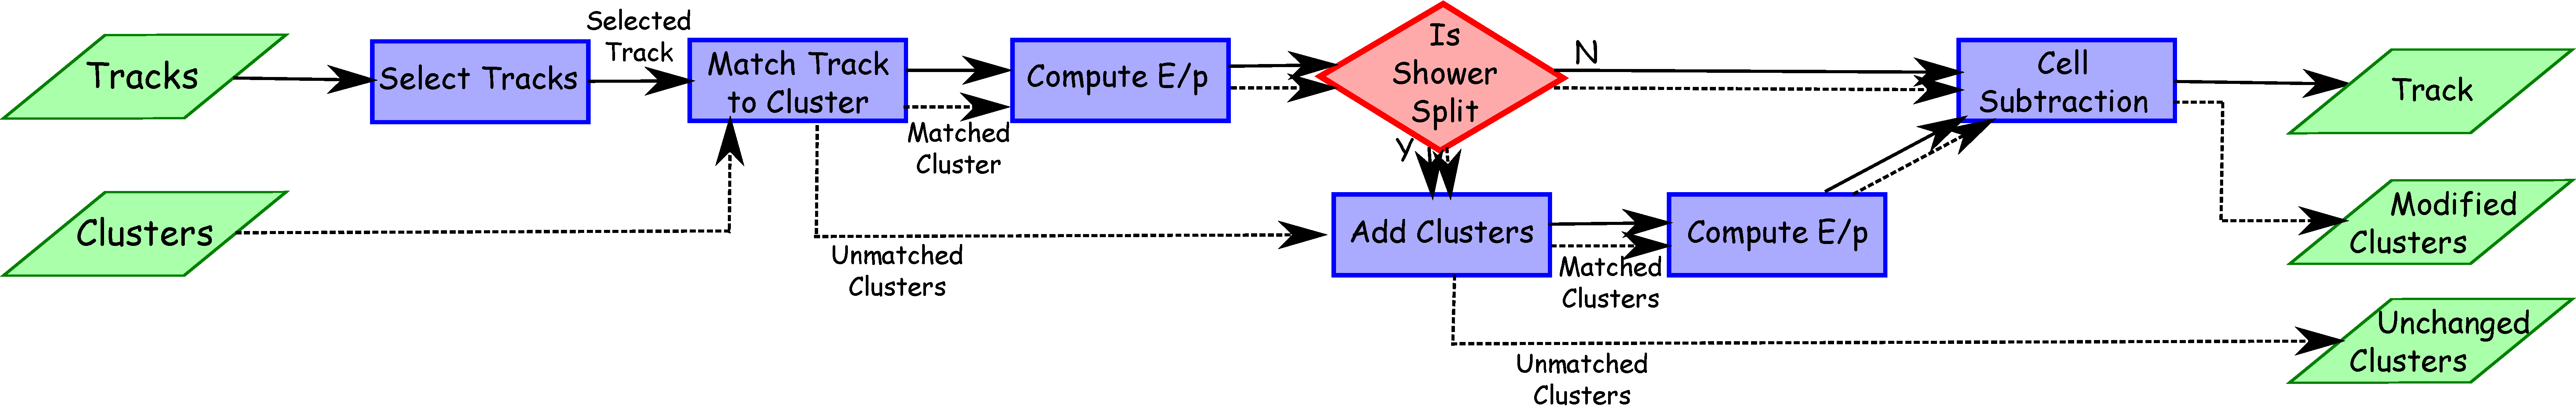
\includegraphics[width=\figwidth]{flowchart.pdf}
  \caption[Flowchart of the steps of the Particle Flow algorithm]{Flowchart of the steps of the Particle Flow algorithm \cite{pflow16}}
  \label{fig:pflowflowchart}
\end{figure}

\subsection{Track selection}

In spite of the clusters the algorithm has some requirements on tracks to be selected to minimize the amount of fake tracks. The requirements are at least 9 hits in the PIXEL and SCT and no missing hits in the PIXEL at all. The tracks have to be in a pseudo-rapidity region of $|\eta|<2.5$ and $\SI{500}{\MeV}<p_T<\SI{40}{\GeV}$.

%check with twiki trackselection



\subsection{Clustering}

The algorithm uses given information from the tracker and the calorimeter as input. The information from the calorimeter is give as topological clusters. The construction of these clusters is briefly described in this chapter to give the reader a basic understanding which input information the algorithm uses.

Each cluster is being constructed around a so called seed cell. A seed cell is a cell for which the deposited energy exceeds the expected noise by four times the standard deviation. If a seed is found all the neighboring cells which exceed the noise by at least two times the standard deviation are added to the cluster. Finally all the cells neighboring these clusters are also added.


\subsection{Matching track to cluster}

The algorithm tries to match every track to one or more calorimeter clusters. First the algorithm tries to match a single best-match topo-cluster to every selected track.
To do so the distances in $\Delta \phi$ and $\Delta \eta$ from the track are extrapolated to the second layer of the EM calorimeter and the topo-clusters. After that the topo-clusters get ranked based on the metric:

\begin{equation}
\Delta R' = \sqrt{\left(\frac{\Delta \phi}{\sigma_{\phi}}\right)^2+\left(\frac{\Delta \eta}{\sigma_{\eta}}\right)^2}
\end{equation}

where $\sigma_{\eta}$ and $\sigma_{\phi}$ refer to the angular topo-cluster width, computed from the standard deviation of the displacemtens of the topo clusters. If the energy in this cluster is greater than or equal to the energy estimated from the track's $p_T$ the algorithm goes to cell subtraction. If the energy in the cluster is smaller than the expected enegery all clusters in a cone of $\Delta R < 0.2$ are matched to the track. In that case R is calculated by the metric:

\begin{equation}
\Delta R = \sqrt{(\Delta \phi)^2 + (\Delta \eta)^2}
\end{equation}

\subsection{Cell Subtraction}

The last step in the Particle Flow algorithm after matching a set of topo-clusters to a track is the cell-wise subtraction of energy deposits to remove remnants and determine which energy depositions belong to the given particle.
If the energy deposited in the set of clusters falls below the expected energy the clusters are simply removed. Otherwise, a cell by cell subtraction is performed.

The first step of the cell subtraction is generating a shower shape from the extrapolated track. Around the extrapolated track rings in $\eta$, $\phi$ space are generated just wide enough to independently contain at least one one cell from the extrapolated position. Furthermore the rings are restricted to one layer and of the same radial size for each layer.
After the generation of rings in each layer the average energy density in each ring is computed and the rings are ranked by energy density in descending order. The layer is not used in any way for this ranking.
The subtraction then starts from the ring with highest energy density and proceeds successively to rings of lower order until the next ring's energy exceeds the remaining expected energy.
If the ring's energy exceeds the energy still to be substracted the energy in each cell is scaled down by the fraction needed to reach the expected energy before the process halts and the remaining cells are removed as remnants.
An example of the process is sketched in figure \ref{fig:sub}. 




\begin{figure}[htbp]
  \centering
  \begin{subfigure}[b]{0.3\figwidth}
    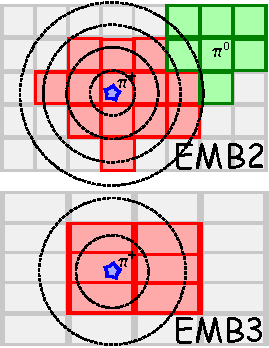
\includegraphics[width=0.25\figwidth]{a}
    \caption{}\label{fig:sub-a}
  \end{subfigure}
  \begin{subfigure}[b]{0.3\figwidth}
    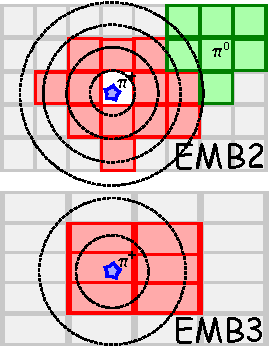
\includegraphics[width=0.25\figwidth]{b}
    \caption{}\label{fig:sub-b}
  \end{subfigure}
  \begin{subfigure}[b]{0.3\figwidth}
    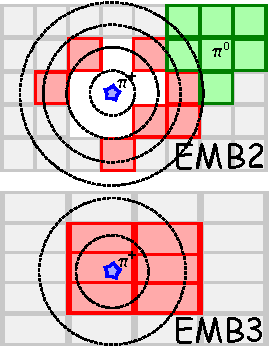
\includegraphics[width=0.25\figwidth]{c}
    \caption{}\label{fig:sub-c}
  \end{subfigure}
  \begin{subfigure}[b]{0.3\figwidth}
    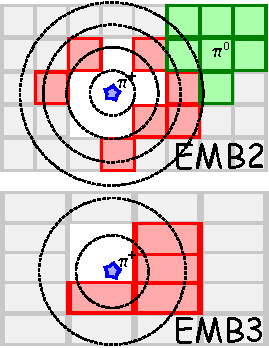
\includegraphics[width=0.25\figwidth]{d}
    \caption{}\label{fig:sub-d}
  \end{subfigure}
    
    
  \begin{subfigure}[b]{0.3\figwidth}
        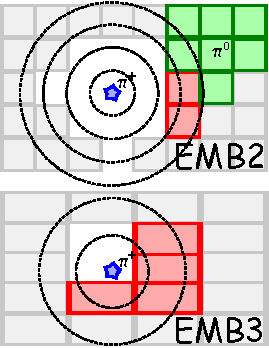
\includegraphics[width=0.25\figwidth]{e}
        \caption{}\label{fig:sub-e}
  \end{subfigure}
  \begin{subfigure}[b]{0.3\figwidth}
        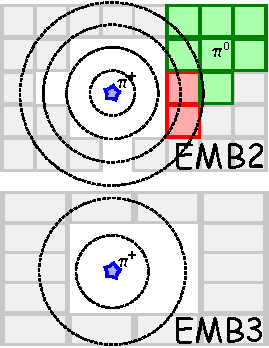
\includegraphics[width=0.25\figwidth]{f}
        \caption{}\label{fig:sub-f}
  \end{subfigure}
  \caption{Example of cell subtraction. In red the depositions originating from the $\pi ^+$ of interest are shown and in green a cluster from a $\pi ^0$ are shown. \cite{pflow16}}
  \label{fig:sub}
\end{figure}

%add a reference here. wildcard there

\subsection{Eflow Rec performance studies}

The Particle Flow manuscript shows the impact of the new algorithm on the angular resolution and on the rejection of pileup jets. This section briefly summarizes the important results of this study. Figure \ref{fig:etarun1} and \ref{fig:phirun1} show the improvements in angular resolution while figure \ref{fig:pileuprun1} displays the increased rejection of fake jets for the new algorithm. LC+JES jets are the jets using the old algorithm and JVF in figure \ref{fig:pileuprun1} refers to the Jet Vertex Fraction representing the amount of energy in the jet originating from the original vertex.

The plots clearly demonstrate that Particle Flow does improve the angular resolution in low $p_T$ regions while having no drawback for higher $p_T$ regions. The pileup contribution is also mediated massively even in comparison to the usage of a cut on the JVT. The region of effect is restricted to $|\eta|<\num{2.5}$ because only this region of pseudorapidity is covered by the Inner Detector. Only the momentum resolution shown in figure \ref{fig:ptrun1} worsens using the old reconstruction for high $p_T$ regions.
%JVT sentence
\begin{figure}[h]
  \centering
  \begin{subfigure}[b]{0.5\figwidth}
  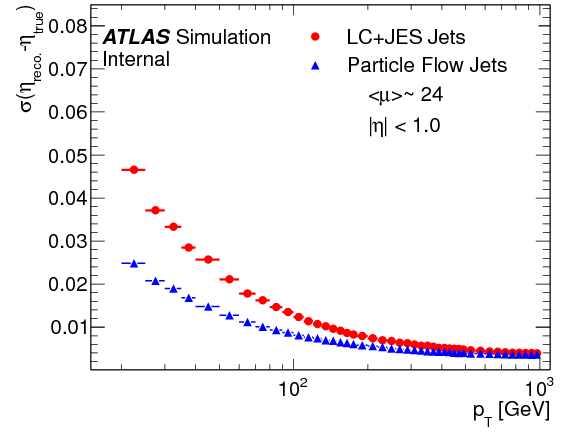
\includegraphics[width=0.5\figwidth]{etarun1.png}
  \caption[Improvements in $\eta$ resolution for Particle Flow Jets]{Improvements in $\eta$ resolution for Particle Flow Jets \cite{pflow16}}
  \label{fig:etarun1}
  \end{subfigure}
  \begin{subfigure}[b]{0.5\figwidth}
  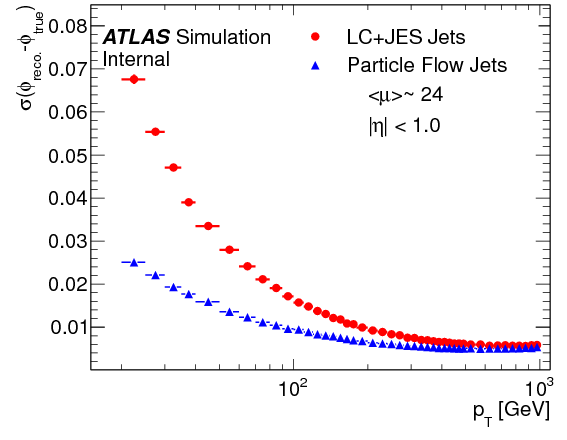
\includegraphics[width=0.5\figwidth]{phirun1.png}
  \caption[Improvements in $\phi$ resolution for Particle Flow Jets]{Improvements in $\phi$ resolution for Particle Flow Jets \cite{pflow16}}
  \label{fig:phirun1}
  \end{subfigure}
\end{figure}

\begin{figure}[h]
  \centering
  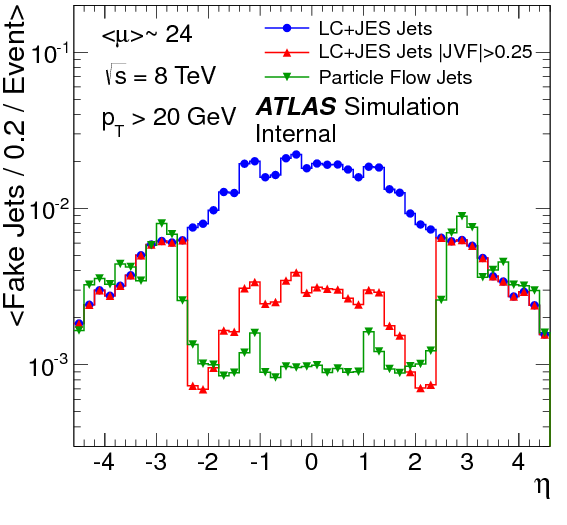
\includegraphics[width=0.8\figwidth]{pileuprun1.png}
  \caption[Pileup comparison of EM-Topo Jets and Particle Flow jets]{Pileup comparison of EM-Topo Jets and Particle Flow jets \cite{pflow16}}
  \label{fig:pileuprun1}
\end{figure}

\begin{figure}
\centering
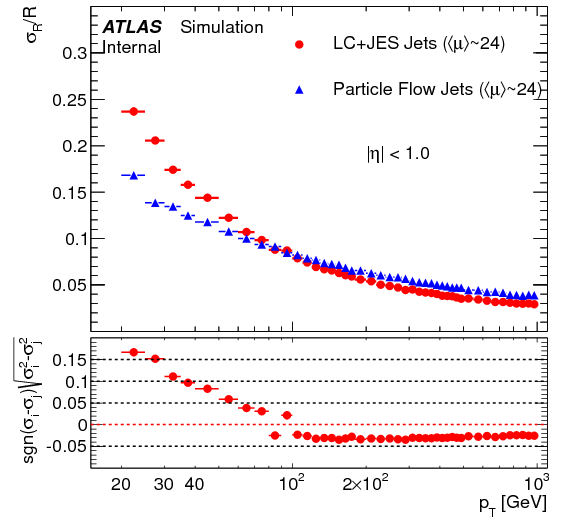
\includegraphics[width=0.8\figwidth]{ptrun1.png}
\caption[Momentum resolution of Particle Flow]{Momentum resolution of Particle Flow jets \cite{pflow16}}
\label{fig:ptrun1}
\end{figure}



\subsection{Recent updates in eflowrec}

The description of the Particle Flow algorithm given in this thesis is based on the analysis of Run 1 data and some recent changes to the algorithm are described in this section.


%Here I want to explain what tools are used for PFlow already and what tools are %missing.
%Then I should focus on which tools have been implicitly upgraded
%Problematic right now are the cleaning the trigger matching the pileup reweithing %and the complete JES